\section{Actividades y Metodología}

%Localización física y ubicación de instalaciones:

El proyecto se llevará a cabo en la Facultad de Ingeniería de la Universidad Nacional de La Plata.
Los ensayos necesarios se realizarán en el Área Técnica de Electrónica e Instrumental (ATEI)
del Departamento de Electrotecnia de la Facultad de Ingeniería de la UNLP.
Se realizarán consultas semanales con el tutor para el seguimiento del desarrollo del proyecto y
revisión de las decisiones tomadas por el equipo de trabajo.

Para alcanzar las metas y los objetivos propuestos, se realizarán las siguientes actividades:

\subsection{Estudio de bibliografía y diseño} \label{subsection:estudio_bibliografia}
Con el objetivo de capacitarse, se estudiarán y analizarán aspectos de seguridad, curvas de carga de la batería 
y topologías de conversores de potencia, de acuerdo con los requerimientos del proyecto. 
Se evaluarán las diferentes alternativas posibles y, en base a su complejidad y a su costo,
se elegirá la solución más adecuada para el logro de los objetivos. 

Se realizarán simulaciones en SPICE (programa de simulación con énfasis en circuitos integrados),
separando el proceso en 4 partes:
\begin{itemize}
    \item Fuente conmutada: Convierte la tensión alterna de la red doméstica en una tensión continua.
    \item Fuente de corriente: Brinda una corriente constante a la batería durante la primera etapa de carga.
    \item Circuito de control: Alterna entre las etapas de carga.
    \item Circuito de protección: Protege a la batería en caso de cortocircuito.
\end{itemize}

En la Figura \ref{fig:esquema_cargador} se puede observar un esquema en bloques del cargador.
El circuito de la fuente conmutada está compuesto por los bloques de rectificación, filtrado y conversión DC-DC.
El controlador se encarga de generar una señal PWM en base a la tensión y la corriente de la batería.
La referencia es una señal de corriente ya que la tensión nominal del cargador es fija.
El circuito de protección está integrado en el bloque de control.

Para disminuir las pérdidas de potencia en la etapa de corriente constante y obtener una mayor eficiencia, se modificó la estructura del cargador con respecto al diseño original. 
En primera instancia, para mantener la tensión a la salida del conversor en 42V, se propuso un ciclo de trabajo constante 
con el cual la caída de tensión en la etapa de control de corriente generaba una disipación de potencia excesiva.
Modificando el circuito de conversión que controla tanto la corriente como la tensión se evita una etapa posterior limitadora de corriente.

%incluir esquema de cargador
\begin{figure}
    \centering
    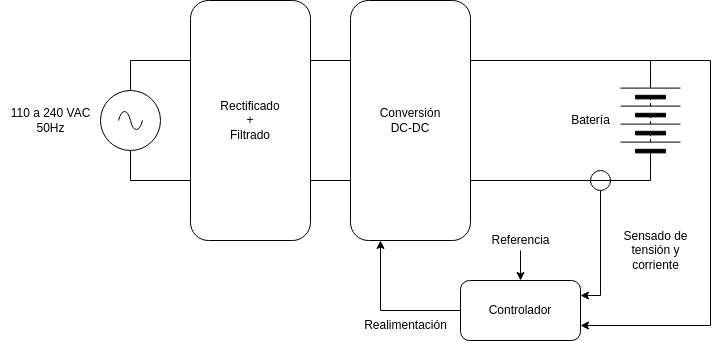
\includegraphics[width=\textwidth]{images/esquema_cargador_v2.png}
    \caption{Esquema del cargador}
    \label{fig:esquema_cargador}
\end{figure}

Se realizará un análisis crítico de las primeras simulaciones y, en base a los resultados obtenidos, 
se corregirán los circuitos propuestos. 
Esta etapa finaliza con la presentación del informe parcial. 

\subsection{Simulaciones}
El circuito fue diseñado y probado en LTspice \cite{ltspice}, con el fin de verificar el diseño.
El proceso hasta el día de la fecha podría dividirse en las siguientes etapas:
\begin{enumerate}
    \item Simulación del conversor.
    \item Simulación del rectificador de entrada.
    \item Simulación del circuito de control.
    \item Simulación de distintos modelos de batería.
\end{enumerate}

En las siguientes secciones se detallarán cada una de estas etapas,
enumerando los problemas encontrados y las soluciones propuestas.

\subsubsection{Simulación del conversor}
El primer paso de diseño fue la elección de una topología de conversión DC-DC.
Esta etapa introduce aislación a partir de un transformador de alta frecuencia,
disminuyendo el coste, tamaño y peso respecto a uno de baja frecuencia en base al núcleo magnético necesario.
Como se requiere una única tensión de salida se evita utilizar múltiples devanados.
El conversor debe alcanzar una potencia máxima de 300W y debe ser lo más sencillo posible para evitar un costo elevado. 

La topología flyback es de baja complejidad al estar integrada por muy pocos componentes. 
Como desventajas, el tamaño del núcleo del transformador se incrementa con la potencia requerida y en bornes del
interruptor presenta una tensión igual al doble de la tensión máxima de entrada.
En aplicaciones típicas se alcanzar valores de hasta 150W.

La topología forward con un solo switch disminuye el tamaño del núcleo del transformador ya que la energía no necesita almacenarse en el entrehierro.
Como desventajas, al igual que el flyback presenta alta tensión en bornes del interruptor y se eleva el costo debido al agregado de la bobina de filtrado.
La topología forward con dos switches reduce la tensión en bornes del interruptor a la mitad respecto a la de un solo switch (y con ello la disipación de potencia por switch), 
pero el circuito de excitación de uno de los transistores queda flotante respecto a masa. 
La topología con un solo switch admite una potencia de salida entre 150-250W y con 2 switches se eleva a 500W \cite{mohan}\cite{hart}. 
En base a los criterios definidos inicialmente se eligió el conversor forward con dos switches como topología de conversión DC-DC. 

El principal problema que presentó la utilización de este conversor fue que las señales que controlan a los switches son poco convencionales.

\subsubsection{Simulación del rectificador de entrada AC-DC}
Una vez definido el circuito de conversión DC-DC, se procedió a analizar los requisitos de la tensión de entrada. 
Los circuitos rectificadores AC-DC permiten convertir una tensión alterna en una tensión continua.

Rectificador de media onda u onda completa

Si bien el rectificador de media onda es más simple ya que cuenta con un menor número de diodos, existen muchas ventajas del rectificador de onda completa frente al de media onda. 
La primera de ellas es que la corriente media del generador de alterna(alimentación) es nula, lo cual beneficia a los transformadores. 
La segunda se basa en el hecho de que para una misma carga, la tensión de rizado pico a pico para el rectificador de onda completa es aproximadamente la mitad que para el rectificador de media onda. 
Esto se debe a que en el circuito de onda completa, el tiempo durante el que se descarga el capacitor es menor que en el circuito de media onda debido a la onda sinusoidal rectificada de la segunda mitad de cada período. 

Por todos estos motivos se decidió implementar un rectificador de onda completa.

Rectificador de onda completa en puente o con toma media

En puente

Presenta la caída de tensión de 2 diodos entre el generador y la carga. 
La tensión máxima en un diodo polarizado en inversa es el valor pico del generador.

Transformador de toma media

Sólo presenta la caída de tensión de un diodo entre el generador y la carga. 
Para una misma potencia entregada por el generador, los diodos consumen potencia y disminuyen la corriente y potencia que absorbe la carga. 
La tensión máxima en un diodo polarizado en inversa es el doble del valor pico del generador.
El transformador proporciona aislamiento eléctrico entre el generador y la carga. 

Como la reducción de tensión a la salida no es significativa en esta aplicación, y el puente de diodos se puede implementar con un pequeño integrado, con el objetivo de disminuir el tamaño del circuito se decidió evitar el transformador y utilizar un rectificador de onda completa tipo puente.

Filtrado
% ¿No usamos bobina?
El filtro pasa bajos compuesto por una red LC permite disminuir el rizado, es decir, la componente de alterna de la señal rectificada. 
Como resultado se logra una tensión de salida aproximadamente continua.
El capacitor mantiene la tensión de salida en un nivel constante y la bobina suaviza la corriente del rectificador y reduce la corriente de pico en los diodos. 

Para disminuir el número de componentes se decidió utilizar únicamente un capacitor en paralelo con la capacidad suficiente para obtener una tensión continua.

Rectificación controlada

Los tiristores son interruptores electrónicos controlados que son activados por una señal externa. 
Poseen 3 terminales: ánodo, cátodo y puerta. Presentan altos valores nominales de corriente y tensión. Soportan altas corrientes y altas tensiones de bloqueo. 
Un ejemplo de tiristores con los rectificadores controlados de silicio(SCR). Para que conduzcan se los debe polarizar en directa y deben recibir una corriente de puerta. 
Al entrar en conducción no es necesaria la señal de puerta para mantener la corriente de ánodo. 
El SCR continuará conduciendo siempre que la corriente de ánodo sea positiva y esté por arriba de un valor mínimo. 
Mediante conmutadores controlados como los SCR se controla la tensión de salida en un rango limitado de variación, ajustando el ángulo de disparo de cada SCR. 
El ángulo de disparo es el intervalo angular entre la polarización directa del SCR y la aplicación de la señal de puerta. 
Si el ángulo de disparo es 0, el comportamiento es igual al de un rectificador no controlado con diodos. 

Se decidió utilizar rectificación no controlada ya que no se necesita una tensión específica a la salida y el costo de complejizar el diseño con el agregado de SCRs y un circuito dedicado de disparo no aporta ningún beneficio significativo.

\subsubsection{Simulación del circuito de control}
Esta etapa fue la mas extensa en diseñar debido a su complejidad. Inicialmente solo debía realimentar la tensión de salida
y generar la señal PWM en base a esta, pero en base a los cambios descritos en la sección \ref{subsection:estudio_bibliografia}
se separó su diseño en tres etapas:

\begin{enumerate}
    \item Compensador y generador PWM
    \item Selector de modo de funcionamiento
    \item Controlador para los switches
\end{enumerate}

La primer etapa se implementó en base a las topologías descritas en \cite{mohan}. Se puede observar,
en la figura \ref{fig:esquema_compensador}, un modelo simplificado del circuito.

\begin{figure}
    \centering
    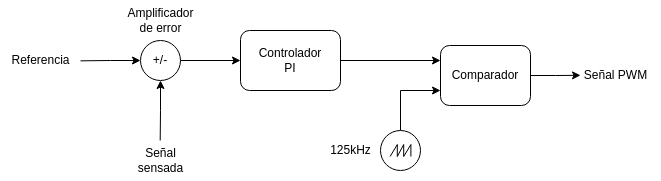
\includegraphics[width=\textwidth]{images/compensador.png}
    \caption{Esquema del compensador y el generador de señal PWM}
    \label{fig:esquema_compensador}
\end{figure}

Los parámetros del bloque proporcional-integrador (PI) fueron definidos a partir de valores típicos obtenidos de \cite{mohan}
y posteriormente ajustados para que el circuito funcione en las condiciones de la aplicación.
La frecuencia de switching es definida por la frecuencia de la señal de diente de sierra y también se tomó un valor típico.

\begin{figure}
    \centering
    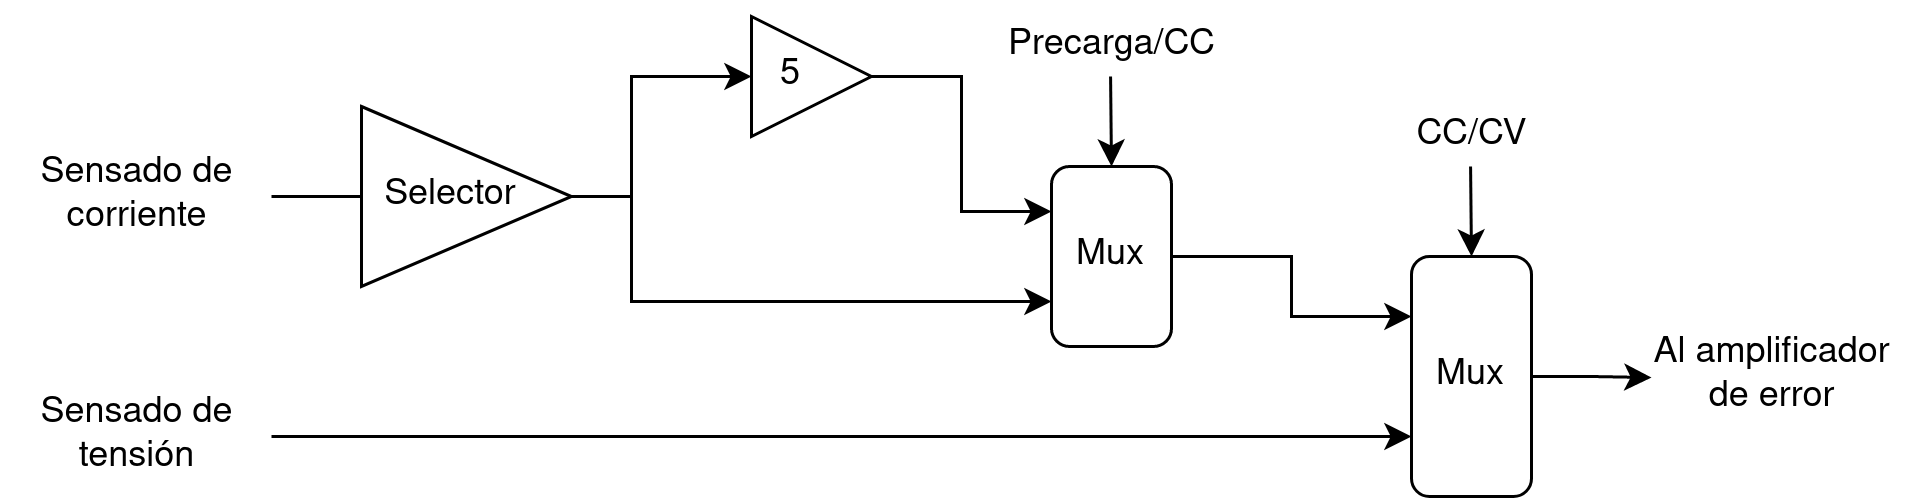
\includegraphics[width=\textwidth]{images/selector.png}
    \caption{Esquema del selector de modo}
    \label{fig:esquema_selector}
\end{figure}

Una vez diseñado el compensador, se procedió a diseñar el circuito de cambio de modo (Precarga, tensión constante y corriente constante).
En la figura \ref{fig:esquema_selector} se puede observar el esquema de este circuito.

Las señales de tensión y corriente están normalizadas con respecto a sus valores nominales.
Un amplificador de ganancia variable actúa como selector de corriente de salida,
modificando la amplitud de la señal de control de dicha variable.
La selección entre el modo de precarga y el modo de corriente constante se hace comparando el nivel de tensión de la batería
con una señal de referencia, siendo el segundo modo activado una vez que la tensión supera los 30V.
El bloque de ganancia 10 tiene como objetivo amplificar la señal de control, ya que la corriente de salida para el modo
de precarga es 10 veces mas chica que la de corriente constante.

La normalización de las señales nombrada anteriormente permite que la selección de la señal del último multiplexor
se haga en base a cual es la mayor de las dos. Esto, visto desde una perspectiva general, permite establecer un límite
tanto de tensión como de corriente de salida, lo cual es importante porque representa la base del método de carga.

Finalmente, para la selección de un controlador para los MOSFETs se tuvieron en cuenta algunos parámetros como
la tensión máxima de entrada, frecuencia de switching y sincronización de las señales,
pero no se logró hallar un controlador adecuado para esta aplicación.
El principal motivo fue que los controladores convencionales generan señales alternadas mediante el método de bootstrapping \cite{hart},
lo cual no sirve para la topología elegida. Esto, combinado con el elevado nivel de tensión en la entrada,
llevó a la búsqueda de otros métodos de control; por eso, se diseñó un controlador propio que se adaptara
a las necesidades del proyecto, cuyo diagrama puede observarse en la figura \ref{fig:driver}.

\begin{figure}
    \centering
    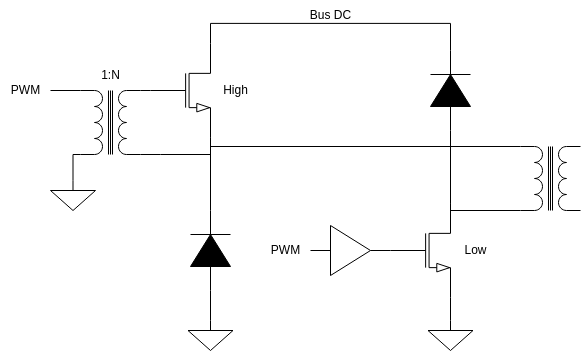
\includegraphics[width=\textwidth]{images/driver.png}
    \caption{Esquema del controlador de los MOSFETs}
    \label{fig:driver}
\end{figure}

\subsubsection{Simulación de distintos modelos de batería}
Para que las simulaciones permitan obtener resultados fiables se buscó un modelo apropiado para la batería.
El primer modelo consta de una resistencia variable a partir de los datos obtenidos de los ensayos. 
Este componente representa la resistencia interna de la batería, que es responsable de la caída de tensión instantánea que se produce ante un escalón en la intensidad demandada.

El siguiente modelo propuesto añade un capacitor de muy alto valor en serie con la resistencia variable,
el cual representa la capacidad de almacenar carga de la batería.
El modelo actual es un modelo dinámico donde los valores de los componentes no son fijos,
sino que dependen de las condiciones de funcionamiento de la batería: estado de carga y funcionamiento en carga o descarga.

El circuito de la izquierda modela la resistencia interna de la batería y el comportamiento transitorio ante distintas cargas.
Por otro lado, el circuito de la derecha modela la capacidad de almacenamiento de energía de la batería y la carga almacenada durante los procesos de carga o descarga \cite{bateria}.

Respecto al segundo modelo se agregan los siguientes componentes:
\begin{itemize}
    \item Los bloques compuestos por una resistencia y un capacitor en paralelo, que modelan la capacidad en los electrodos de las celdas y
    la resistencia no lineal entre electrodos y electrolito.
    En conjunto modelan las constantes de tiempo corta y larga de la respuesta transitoria de la tensión en la batería\cite{bateria_espanol}.
    \item La fuente de tensión controlada por tensión, que representa la dependencia no lineal entre el estado de carga ($SOC$)
    y la tensión de circuito abierto($V_{OC}$) dependiente del $SOC$.
    \item La fuente de corriente controlada por corriente, representando la corriente de carga que modifica el $SOC$.
\end{itemize}
La tensión que existe en el circuito secundario ($V_{SOC}$) se normaliza de forma que $V_{SOC}=1V$ equivale al $SOC (100\%)$.
La resistencia en paralelo modela la autodescarga de la batería.

\begin{figure}
    \centering
    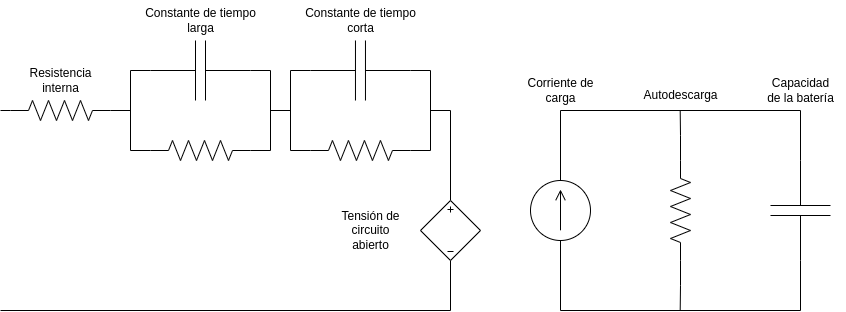
\includegraphics[width=\textwidth]{images/bateria_3.png}
    \caption{Tercer y actual modelo de batería utilizado}
    \label{fig:bateria_3}
\end{figure}

\subsection{Diseños pendientes}
Habiendo desarrollado el cargador casi en su totalidad, aún queda por diseñar el circuito de protección
contra cortocircuitos y el LED indicador. Ambos serán desarrollados durante la segunda parte del proyecto,
debido a su baja complejidad con respecto al resto del circuito.

Inicialmente se planeó implementar un filtro de entrada para evitar (ACA VAS VOS)

\subsection{Implementación}
Se diseñará un circuito impreso y se construirá un prototipo funcional que cumpla con las especificaciones propuestas. 
Debido a que el costo de una batería de litio de las características necesarias es elevado,
se evaluará la posibilidad de realizarlo a escala con una batería de menor tensión y/o capacidad.

\subsection{Validación}
Una vez terminado el proceso de diseño e implementación,
se verificará que el prototipo cumpla con las especificaciones presentadas.
